\section{Fonctionnement}
Comme précisé lors de l'introduction, nous avons décidé d'utiliser des processus et non des threads. Le processus main lance un processus de gestion des feux qui change les feux toutes les 7 secondes. C'est également ce processus qui se charge de récupérer les données de la file de message des bus pour les traiter et ainsi faire passer le bus le plus vite possible. En parallèle, un procesus de gestion des directions s'occupe de générer les voitures, les bus et pour chacune de se mettre en fin de file et attendre le passage au vert s'il n'y est pas. Ce procédé de gestion des directions est effectué pour chaque direction, 4 processus sont donc utilisés.
\newpage
\begin{figure}[htb!]
\centering
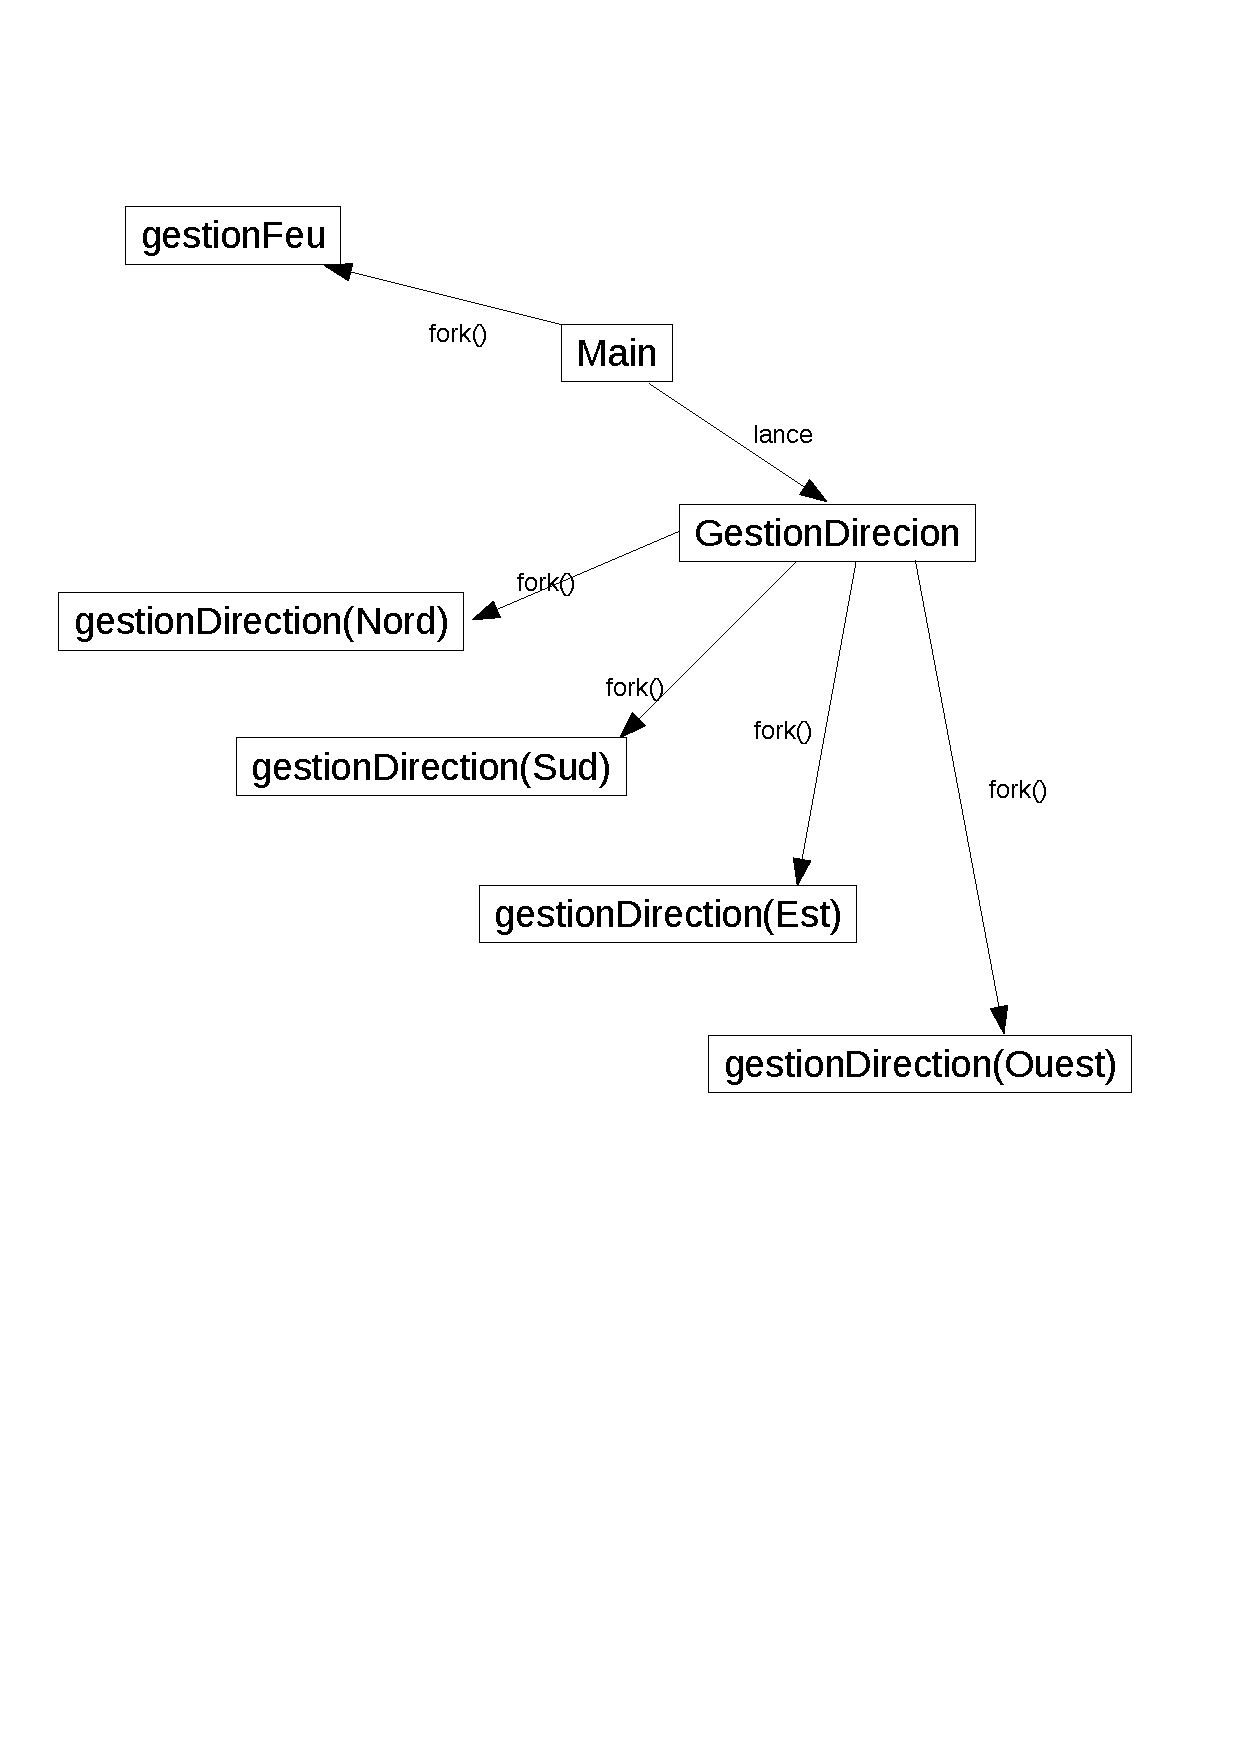
\includegraphics[scale=0.5]{graphe3LO41.pdf}

\caption{Lancement des processus.}
\end{figure}
